\section{Step-by-step example: time-series with anomaly}
\label{S:ExampleDispAnomaly}

This example uses a time series data that mimics displacement data measured on a bridge (synthetic data). 
The baseline switches between a trend stationary to acceleration stationary dynamics during a specific time window to mimic a fictitious anomaly.
The anomalous time windows is of 26 days duration, starting on June 25, 2010.


\subsection{Step 1: start a project}

First, choose the interactive tool by typing \colorbox{light-gray}{\lstinline[basicstyle = \mlttfamily \small, backgroundcolor = \color{light-gray}]!0!}.
Secondly, provide a project name (i.e. \lstinline[basicstyle = \mlttfamily \small, backgroundcolor = \color{light-gray}]!Example_DISP_ANOMALY!).
Then, answer \colorbox{light-gray}{\lstinline[basicstyle = \mlttfamily \small, backgroundcolor = \color{light-gray}]!no!} to indicate that you are not concerned with creating synthetic data.
The next step is to type \colorbox{light-gray}{\lstinline[basicstyle = \mlttfamily \small, backgroundcolor = \color{light-gray}]!0!} to indicate that you aim to load new data.


\subsection{Step 2: load the data}

\begin{figure*}[h!]
\centering
\begin{subfigure}{\linewidth}
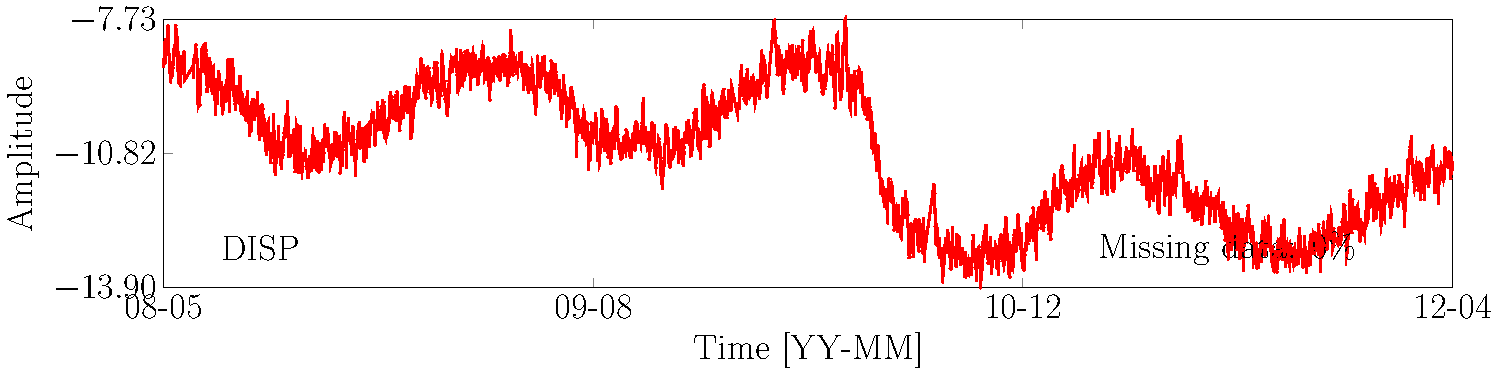
\includegraphics[width=0.9\linewidth]{./docfigs/Example_DISPSIM_ANOMALY/raw/ALL_AMPLITUDES.pdf} 
\caption{Amplitude}
\end{subfigure}
\begin{subfigure}{\linewidth}
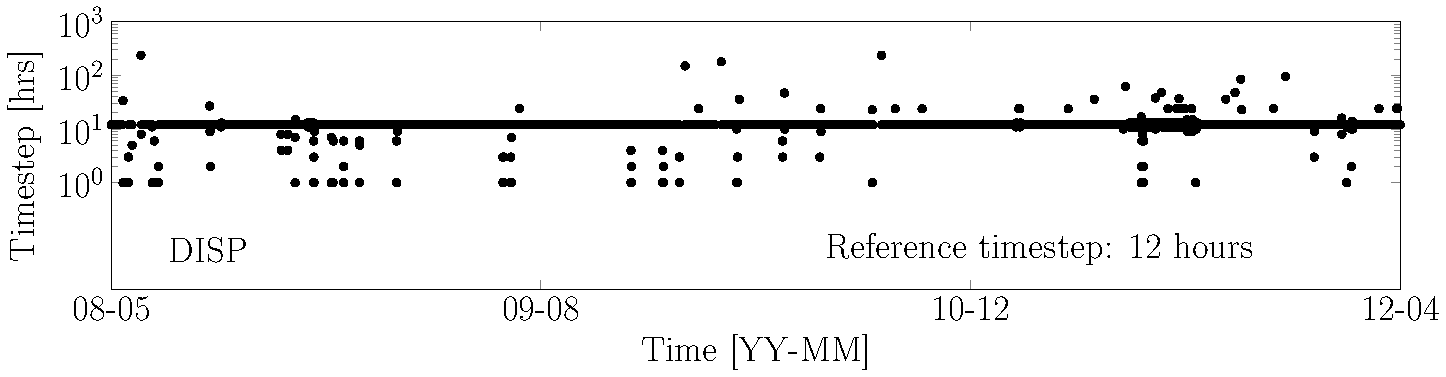
\includegraphics[width=0.9\linewidth]{./docfigs/Example_DISPSIM_ANOMALY/raw/ALL_TIMESTEPS.pdf}
\caption{Timestep}
\end{subfigure}
\begin{subfigure}{\linewidth}
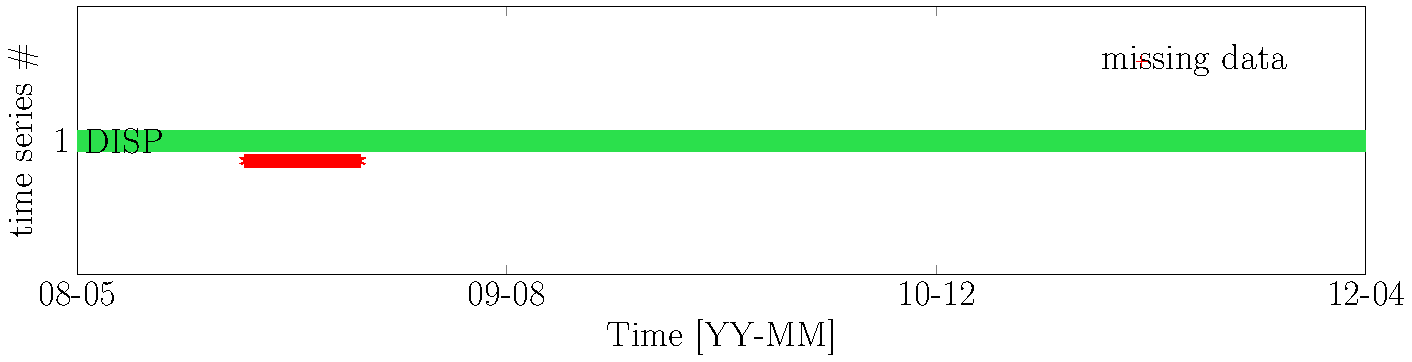
\includegraphics[width=0.9\linewidth]{./docfigs/Example_DISPSIM_ANOMALY/raw/AVAILABILITY.pdf}
\caption{Availability}
\end{subfigure}
\caption{Data used in Section~\ref{S:ExampleDispAnomaly}}.
\label{fig:DataSummaryRaw3}
\end{figure*}


At this stage, a graphical user interface should appear on screen. 
Browse the ``data/csv'' folder to select the csv file named \lstinline[basicstyle = \mlttfamily \small, backgroundcolor = \color{light-gray}]!Example_DISP_ANOMALY_DISP.csv!.
Then, click on the Add button, and then the Done button, as highlighted in Figure~\ref{fig:DataLoadingUIPickFileExample1}.
You will notice that some basic information regarding the loaded time-series, such as the time series index, the reference name and the number of data points are now displayed in the \MATLAB{} command window.
At this time, three \MATLAB{} figures as those represented in Figure~\ref{fig:DataSummaryRaw3} should popup on screen.
The first figure represents in red the data amplitude of each time series data; the second figure represents the data timestep, and the last figure the data availability.
The figures show that data points exist between May 2008 and April 2012 (see Figure~\ref{fig:DataSummaryRaw3}a).
The timestep is non-uniform; it varies from 1 hour to 10 days (see Figure~\ref{fig:DataSummaryRaw3}b). 
The most frequent (i.e referent) time step is 12 hour.
There is no missing data on the displacement time-series.

\subsection{Step 4: configure the model}

First, the program requests the number of model class.
In this example, a change is clearly observed in the data, and we are therefore interested to model non-stationary data and eventually detect the change (i.e. anomaly detection).
In such case, we type \colorbox{light-gray}{\lstinline[basicstyle = \mlttfamily \small, backgroundcolor = \color{light-gray}]!2!} to build a switching model with two model classes.
Then, OpenBDLM asks for the type of block component for the first and second model class. 
The data baseline looks level or trend stationary, and there is a clear yearly periodic pattern superimposed to it.
%The presence of a daily periodic pattern is unclear.
Therefore, we choose \colorbox{light-gray}{\lstinline[basicstyle = \mlttfamily \small, backgroundcolor = \color{light-gray}]![23 31 41]!} for the first model class and \colorbox{light-gray}{\lstinline[basicstyle = \mlttfamily \small, backgroundcolor = \color{light-gray}]![13 31 41]!} for the second model class.
This model considers a trend stationary model with a yearly periodic pattern for the first model class, and an acceleration stationary model with a yearly periodic pattern for the second model class.
The next step is to define the model parameter constrain between the two model classes. 
Here, it is reasonable to consider that the two model classes only differs in the baseline dynamics, not in the periodic or autoregressive component. 
Therefore, we type \colorbox{light-gray}{\lstinline[basicstyle = \mlttfamily \small, backgroundcolor = \color{light-gray}]![0 1 1]!} to indicate that the two model classes share the same model parameter, except for the baseline component.
The  output on \MATLAB{} command window during interactive model configuration is presented in Listing~\ref{LST:OpenBDLMModelConfigureExample3}.
Type $\dlsh$ to valid.
The model is then built, a \lstinline[basicstyle = \mlttfamily \small, backgroundcolor = \color{light-gray}]!DATA_Example_DISP_ANOMALY.mat! binary data file, a \lstinline[basicstyle = \mlttfamily \small, backgroundcolor = \color{light-gray}]!CFG_DISP_ANOMALY.m! configuration file, as well as a \lstinline[basicstyle = \mlttfamily \small, backgroundcolor = \color{light-gray}]!PROJ_Example_DISP_ANOMALY.mat! project file are created.
The OpenBLDM main menu must appear on the \MATLAB{} command window (see Listing~\ref{LST:OpenBDLMMainMenu}).
Type \colorbox{light-gray}{\lstinline[basicstyle = \mlttfamily \small, backgroundcolor = \color{light-gray}]!Q!} to save and quit.



 \begin{lstlisting}[ frame = single, basicstyle = \mlttfamily \small, caption = { \MATLAB{} command window output during model configuration}, label = LST:OpenBDLMModelConfigureExample3,  float =h!, linewidth=\linewidth, captionpos=b, breaklines=true]
- How many model classes do you want for each time-series? 
     choice >> 2
     
     --------------------------------
     BDLM Component reference numbers
     --------------------------------
     11: Local level 
     12: Local trend 
     13: Local acceleration 
     21: Local level compatible with local trend 
     22: Local level compatible with local acceleration 
     23: Local trend compatible with local acceleration 
     31: Periodic 
     41: Autoregressive process (AR(1)) 
     51: Kernel regression 
     61: Level Intervention 
     --------------------------------

- Model class # 1 

- Identify components for time series #1; e.g. [11 31 41]
     choice >> [23 31 41]

- Model class # 2 

- Identify components for time series #1; e.g. [11 31 41]
     choice >> [13 31 41]

- Identify the shared parameters between the components of the model classes 1 and 2 for time  series #1 ; e.g. [0 1 1]
     choice >> [0 1 1]

     Building model...
     Saving project...
     Project saved in saved_projects/PROJ_Example_DISP_ANOMALY.mat. 
     Printing configuration file...
     Saving data...

     Database saved in data/mat/DATA_Example_DISP_ANOMALY.mat 
     Configuration file saved in config_files/CFG_Example_DISP_ANOMALY.m. 
\end{lstlisting}



\subsection{Step 5: open the configuration file}

After the data loading and the model configuration, a configuration file named \lstinline[basicstyle = \mlttfamily \small, backgroundcolor = \color{light-gray}]!CFG_Example_DISP_ANOMALY.m! configuration file is automatically created and saved in ``config\_files'' folder.
Open the configuration file from \MATLAB{} command line by typing  \colorbox{light-gray}{\lstinline[basicstyle = \mlttfamily \small, backgroundcolor = \color{light-gray}]!edit CFG_Example_DISP_ANOMALY.m!}.
The Model parameters section of the configuration file shows that the model totalizes 12 model parameters, that is 
\begin{gather*}
\bm\theta=\{\sigma_{w, \text{D}}^{TcA,1}, p^{\text{PD1}}_{\text{D}}, \sigma_{w,\text{D}}^{\text{PD1}}, \phi^{AR}_{\text{D}}, \sigma_{w,\text{D}}^{AR}, \\
 \sigma_{w, \text{D}}^{LA,2}, \sigma_{w, \text{D}}^{TcA, 12}, \sigma_{w, \text{D}}^{LA, 21}, \sigma^{1}_{v,\text{D}}, \sigma^{2}_{v,\text{D}}, Z^{11},   Z^{22}\} 
 \end{gather*}
%The default value of the model parameters are assigned  using heuristic knowledge or computed from the data using statistics on the data.
The default model parameters values are 
\begin{gather*}
\bm\theta^{\text{default}}=\{1.5018\times10^{-8}, 365.24, 0, 0.75, 0.075092, \\
1.5018\times10^{-8}, 1.5018\times10^{-8}, 1.5018\times10^{-5}, 0.075092, 0.075092, 0.99986, 0.99986\}.
\end{gather*}
%In the same manner, default value for the initial hidden states are assigned using heuristic knowledge or computed using statistics on the data.
The default initial hidden states mean, covariance  and model probability values for model class 1 are 
\begin{align*}
 \bm \mu^{1,\text{default}}_{0} & = [	-8.72 ,	0    , 	0     ,	5   ,  	0    , 	0       ]^{\intercal}, \text{and} \\
 \text{diag}(\bm\Sigma^{1,\text{default}}_{0})  & = [	9.02  ,	2.26  	, 2.26  ,	9.02  	, 9.02  ,	2.26     ], \text{and} \\
 \pi_{0}^{1,\text{default}} & = 0.5.
\end{align*}
respectively.
The default initial hidden states mean, covariance  and model probability values for model class 2 are 
\begin{align*}
 \bm \mu^{2,\text{default}}_{0} & = [	-8.72 	, 0    , 	0  ,   	5   ,  	0   ,  	0       ]^{\intercal}, \text{and} \\
 \text{diag}(\bm\Sigma^{2,\text{default}}_{0})  & = [	9.02  ,	2.26  	, 2.26  ,	9.02  	, 9.02  ,	2.26    ], \text{and} \\
 \pi_{0}^{2,\text{default}} & = 0.5.
\end{align*}
respectively.



\subsection{Step 6: estimate the hidden states}

Type \colorbox{light-gray}{\lstinline[basicstyle = \mlttfamily \small, backgroundcolor = \color{light-gray}]!OpenBDLM_main('CFG_Example_DISP_ANOMALY.m');!} in the \MATLAB{} command line.
Once, the main menu appears, type  \colorbox{light-gray}{\lstinline[basicstyle = \mlttfamily \small, backgroundcolor = \color{light-gray}]!3!}, then \colorbox{light-gray}{\lstinline[basicstyle = \mlttfamily \small, backgroundcolor = \color{light-gray}]!1!} to estimate the filtered hidden states using the default model parameters and default initial hidden states values.
The value of the log-likelihood is $-409$.
The estimated hidden states are presented in Figure~\ref{fig:DISPSIMANOMALYDefaultDefaultExample3}.

\begin{figure*}[h!]
\centering
\begin{subfigure}{\linewidth}
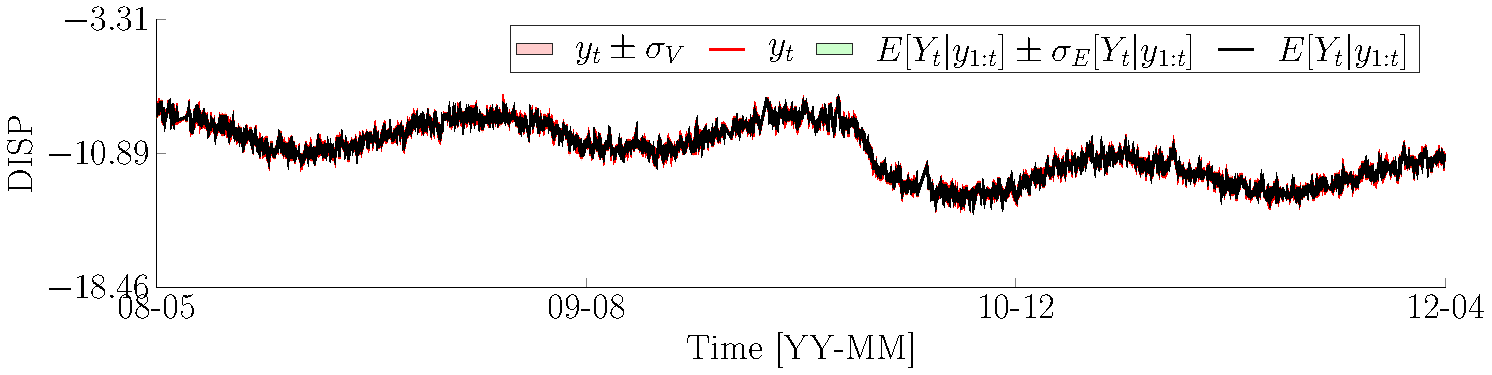
\includegraphics[width=0.9\linewidth]{./docfigs/Example_DISPSIM_ANOMALY/default/DISP_ObservedPredicted.pdf}
\caption{Observed and estimated displacement data}
\end{subfigure}
\begin{subfigure}{\linewidth}
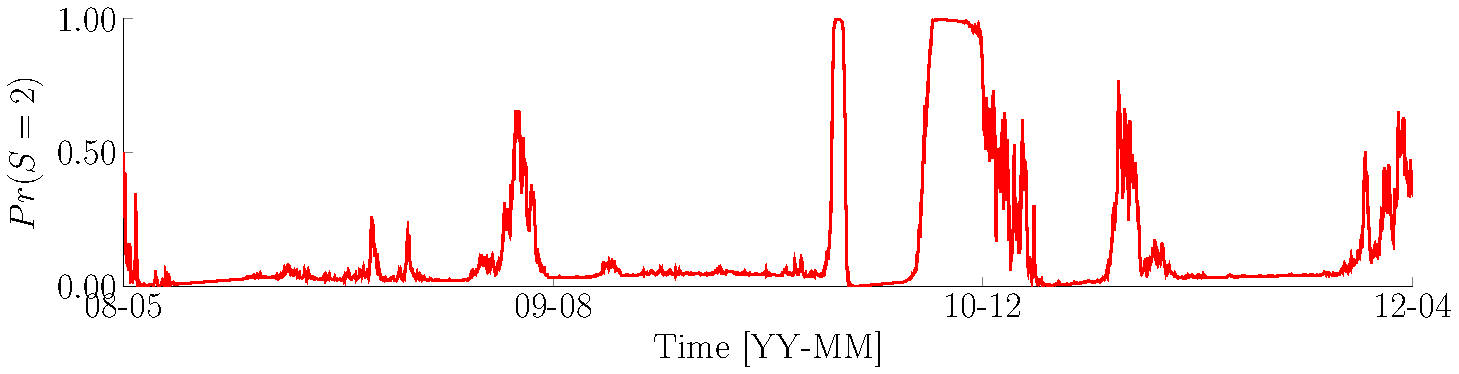
\includegraphics[width=0.9\linewidth]{./docfigs/Example_DISPSIM_ANOMALY/default/ModelProbability.pdf} 
\caption{Estimated probability of anomaly (probability of model class 2)}
\end{subfigure}
\begin{subfigure}{\linewidth}
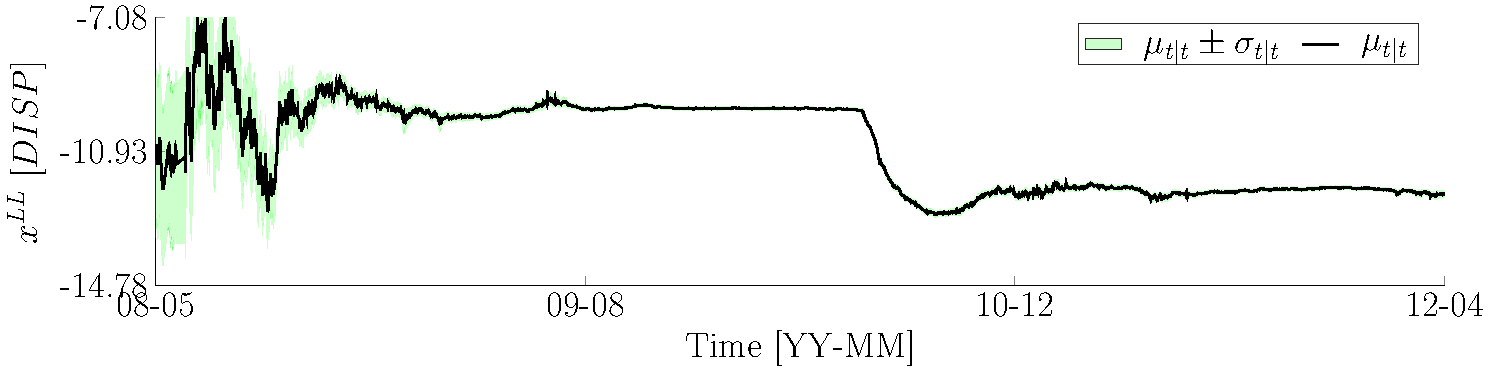
\includegraphics[width=0.9\linewidth]{./docfigs/Example_DISPSIM_ANOMALY/default/DISP_LL_1.pdf} 
\caption{Estimated displacement local level component}
\end{subfigure}
\begin{subfigure}{\linewidth}
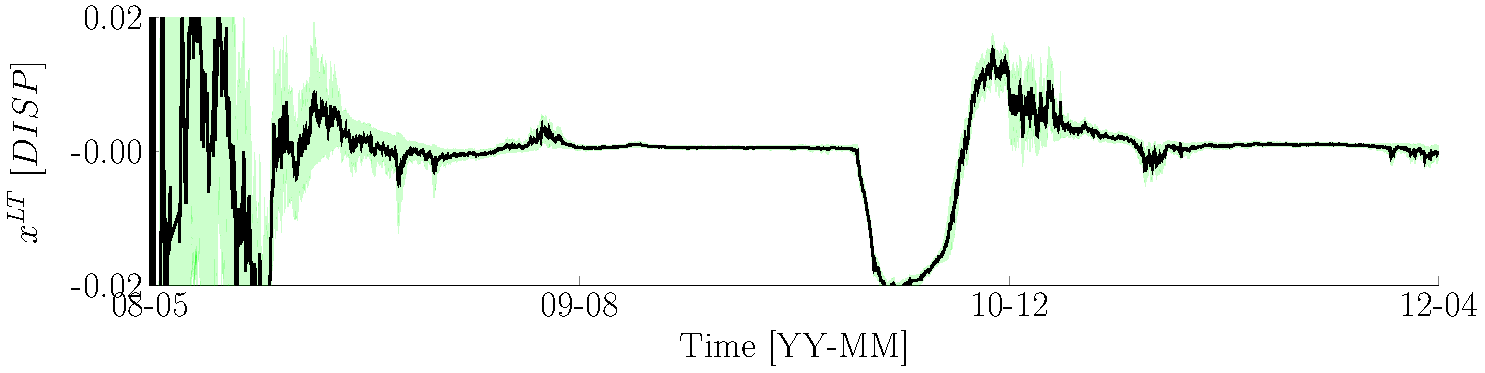
\includegraphics[width=0.9\linewidth]{./docfigs/Example_DISPSIM_ANOMALY/default/DISP_LT_2.pdf}
\caption{Estimated displacement local trend component.}
\end{subfigure}
\begin{subfigure}{\linewidth}
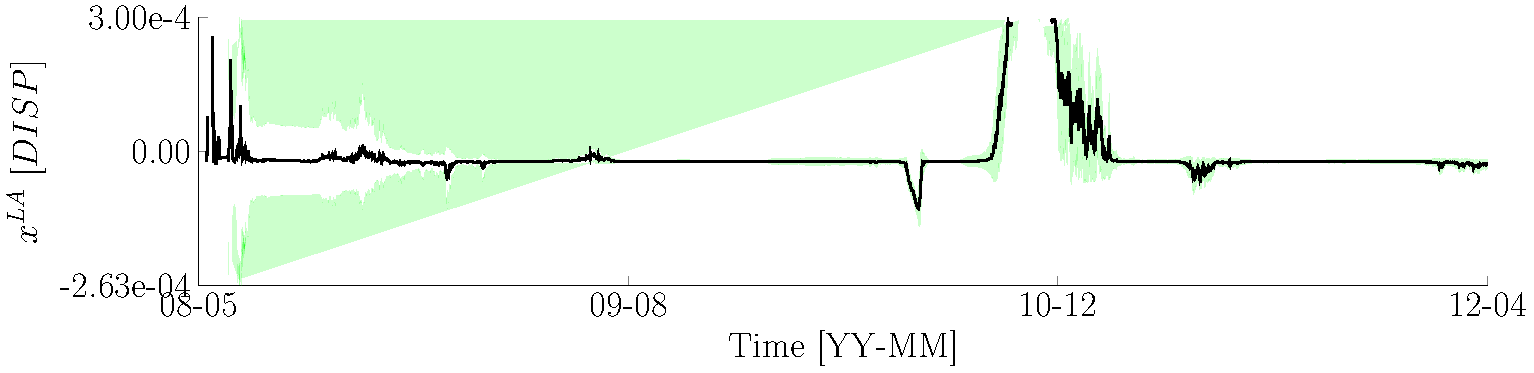
\includegraphics[width=0.9\linewidth]{./docfigs/Example_DISPSIM_ANOMALY/default/DISP_LAc_3.pdf}
\caption{Estimated displacement local acceleration component.}
\end{subfigure}
\end{figure*}
\begin{figure*}[h!]
\ContinuedFloat
\begin{subfigure}{\linewidth}
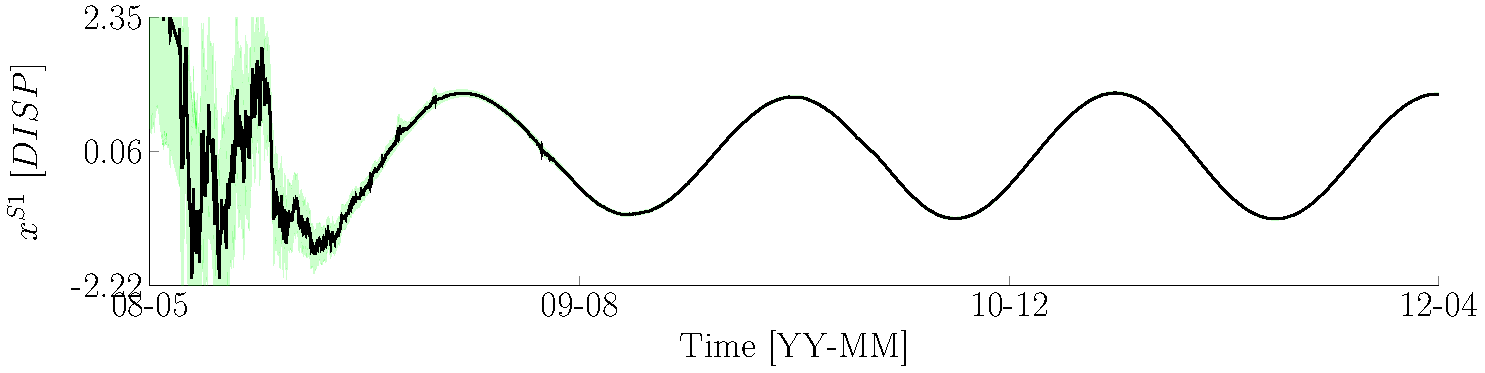
\includegraphics[width=0.9\linewidth]{./docfigs/Example_DISPSIM_ANOMALY/default/DISP_S1_4.pdf}
\caption{Estimated displacement yearly periodic component (first hidden state)}
\end{subfigure}
\begin{subfigure}{\linewidth}
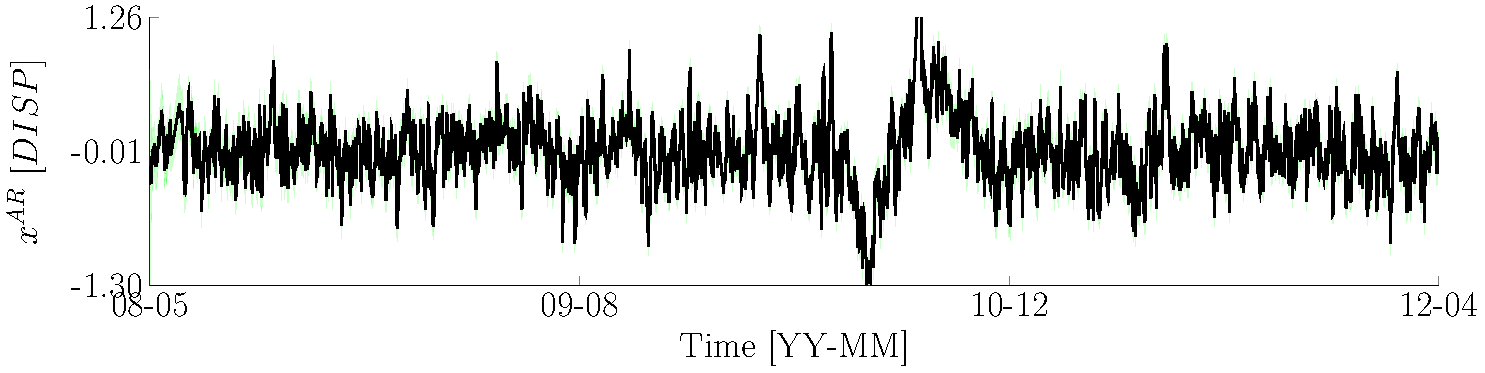
\includegraphics[width=0.9\linewidth]{./docfigs/Example_DISPSIM_ANOMALY/default/DISP_AR_6.pdf} 
\caption{Estimated displacement autoregressive component}
\end{subfigure}
\caption{Estimated results using OpenBDLM default model parameters and default initial hidden states. The hidden states are estimated from the data presented in Figure~\ref{fig:DataSummaryRaw3}a. The solid line and shaded area represent the mean and standard deviation of the estimated hidden states, respectively.}
\label{fig:DISPSIMANOMALYDefaultDefaultExample3}
\end{figure*}

\subsection{Step 7: estimate the model parameters from the data}

Type \colorbox{light-gray}{\lstinline[basicstyle = \mlttfamily \small, backgroundcolor = \color{light-gray}]!OpenBDLM_main('CFG_Example_DISP_ANOMALY.m');!} in the \MATLAB{} command line.
Once, the main menu appears, type  \colorbox{light-gray}{\lstinline[basicstyle = \mlttfamily \small, backgroundcolor = \color{light-gray}]!1!}, then \colorbox{light-gray}{\lstinline[basicstyle = \mlttfamily \small, backgroundcolor = \color{light-gray}]!1!} to estimate the model parameters using Newton-Raphson (type  \colorbox{light-gray}{\lstinline[basicstyle = \mlttfamily \small, backgroundcolor = \color{light-gray}]!1!} to use the Stochastic Gradient instead).
The model parameters learning procedure should start (see for example Listing~\ref{LST:OpenBLDMModelParameterLearning}).
Note that, by default, OpenBDLM considers that the parameters $P^{\text{PD1}}$, $\sigma_{w}^{\text{PD1}}$ are known.
Therefore, there are ten model parameters to be learned from the data in this example.
The estimation of the model parameters may take several hours.
Therefore, press combinations \colorbox{light-gray}{\lstinline[basicstyle = \mlttfamily \small, backgroundcolor = \color{light-gray}]!Ctrl!} + \colorbox{light-gray}{\lstinline[basicstyle = \mlttfamily \small, backgroundcolor = \color{light-gray}]!c!} to abort the process.
Once the algorithm is converged, the optimized model parameters values should be close to  \footnote{Note that it is possible to get slightly different value of parameters with the same performance.}
\begin{gather*}
\bm\theta^{\text{*}}=\{0, 365.24, 0, 0.75, 0.213, \\
0.001, 8.1224\times10^{-6}, 1.5018\times10^{-5}, 0.10671, 0.10671, 0.99997, 0.99957\}.
\end{gather*}


\subsection{Step 8: estimate the hidden states using the optimized model parameters values}

In the ``examples/Example\_DISP\_ANOMALY'' folder, there is a configuration file named \lstinline[basicstyle = \mlttfamily \small, backgroundcolor = \color{light-gray}]!CFG_Example_DISP_ANOMALY_optim.m! that contains optimized model parameters estimated using the Newton-Raphson algorithm.
Copy and paste \lstinline[basicstyle = \mlttfamily \small, backgroundcolor = \color{light-gray}]!CFG_Example_DISP_ANOMALY_optim.m! from  the ``examples/Example\_DISP\_ANOMALY'' subfolder  to the ``config\_files'' folder.
Type \colorbox{light-gray}{\lstinline[basicstyle = \mlttfamily \small, backgroundcolor = \color{light-gray}]!OpenBDLM_main('CFG_Example_DISP_ANOMALY_optim.m');!} in the \MATLAB{} command line to load the configuration file  \lstinline[basicstyle = \mlttfamily \small, backgroundcolor = \color{light-gray}]!CFG_Example_DISP_ANOMALY_optim.m!.
Once the main menu appears, type  \colorbox{light-gray}{\lstinline[basicstyle = \mlttfamily \small, backgroundcolor = \color{light-gray}]!3!}, then \colorbox{light-gray}{\lstinline[basicstyle = \mlttfamily \small, backgroundcolor = \color{light-gray}]!1!} to estimate the filtered hidden states using the optimized model parameters and default initial hidden states values.
The value of the log-likelihood is now $172$.
The estimated hidden states are presented in Figure~\ref{fig:DISPSIMANOMALYOptimizedDefaultExample3}.

\begin{figure*}[h!]
\centering
\begin{subfigure}{\linewidth}
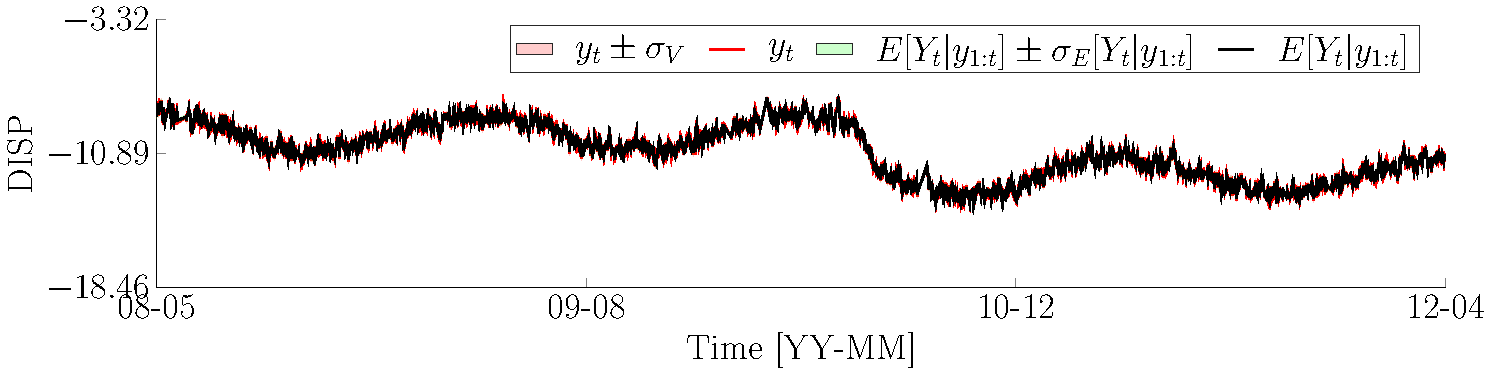
\includegraphics[width=0.9\linewidth]{./docfigs/Example_DISPSIM_ANOMALY/optim_param_default_initialhiddenstate/DISP_ObservedPredicted.pdf}
\caption{Observed and estimated displacement data}
\end{subfigure}
\begin{subfigure}{\linewidth}
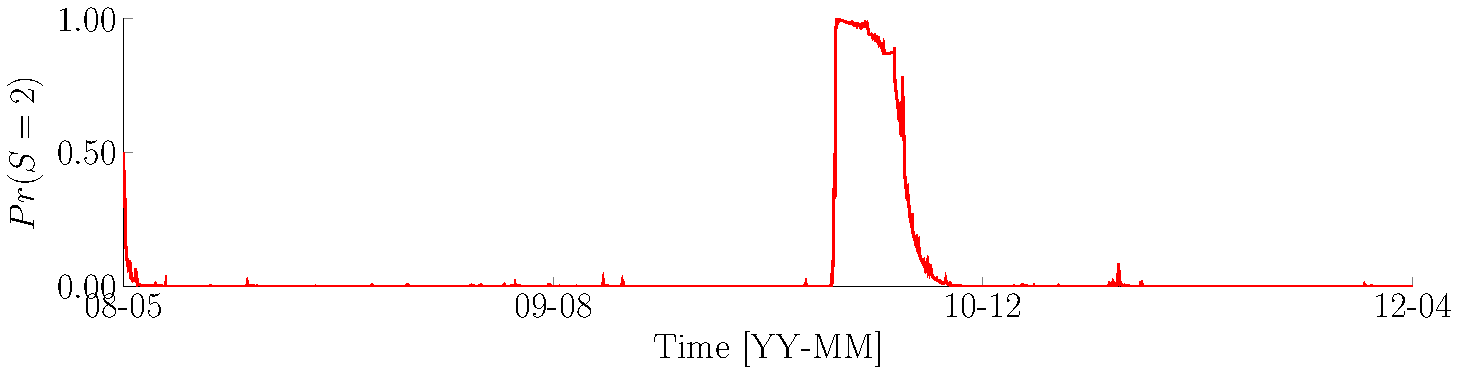
\includegraphics[width=0.9\linewidth]{./docfigs/Example_DISPSIM_ANOMALY/optim_param_default_initialhiddenstate/ModelProbability.pdf} 
\caption{Estimated probability of anomaly (probability of model class 2)}
\end{subfigure}
\begin{subfigure}{\linewidth}
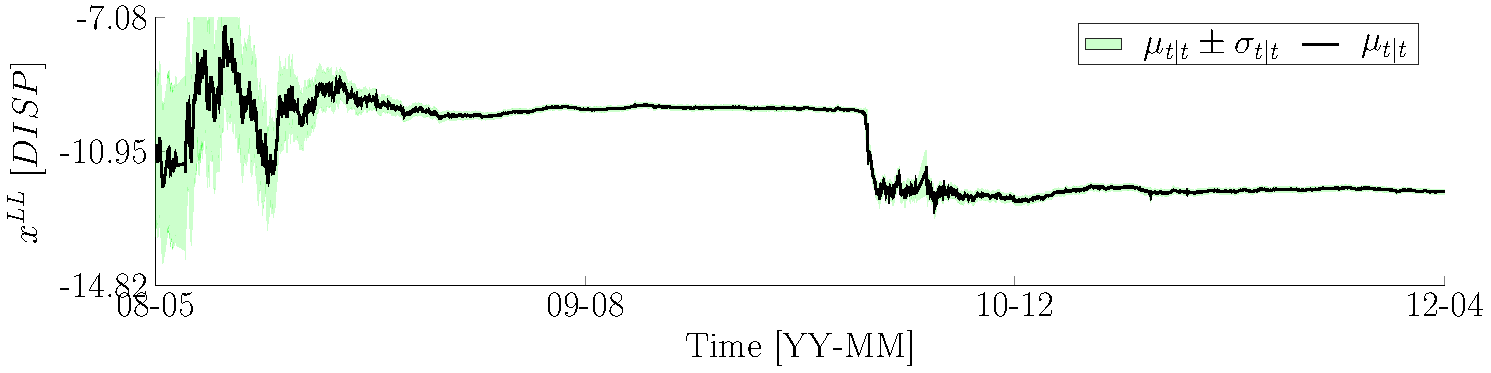
\includegraphics[width=0.9\linewidth]{./docfigs/Example_DISPSIM_ANOMALY/optim_param_default_initialhiddenstate/DISP_LL_1.pdf} 
\caption{Estimated displacement local level component}
\end{subfigure}
\begin{subfigure}{\linewidth}
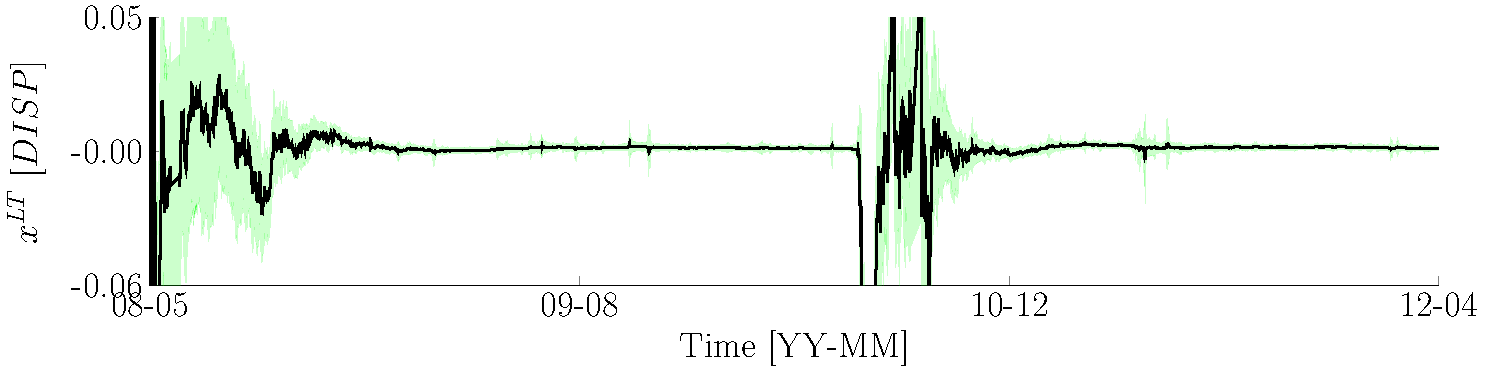
\includegraphics[width=0.9\linewidth]{./docfigs/Example_DISPSIM_ANOMALY/optim_param_default_initialhiddenstate/DISP_LT_2.pdf}
\caption{Estimated displacement local trend component.}
\end{subfigure}
\begin{subfigure}{\linewidth}
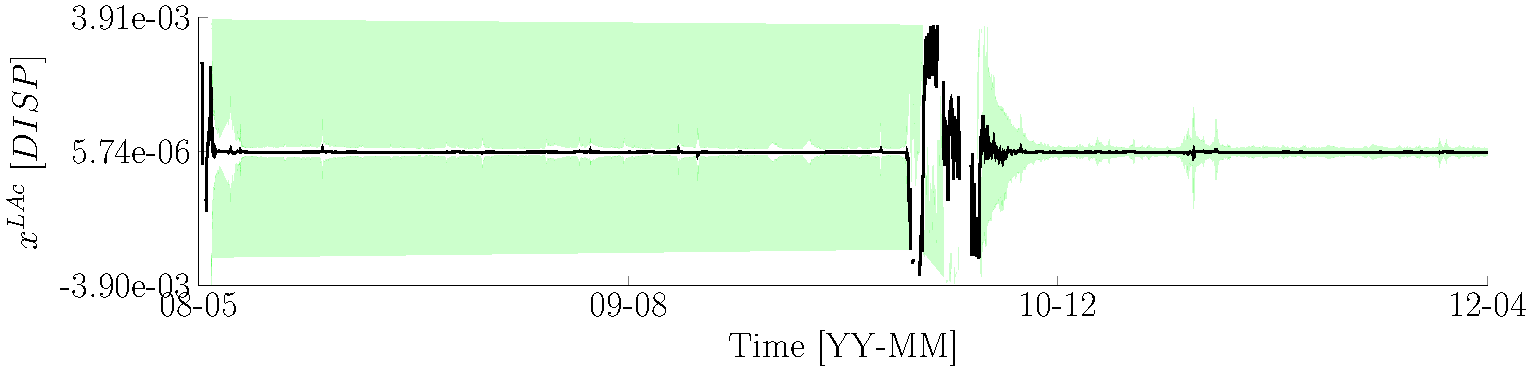
\includegraphics[width=0.9\linewidth]{./docfigs/Example_DISPSIM_ANOMALY/optim_param_default_initialhiddenstate/DISP_LAc_3.pdf}
\caption{Estimated displacement local acceleration component.}
\end{subfigure}
\end{figure*}
\begin{figure*}[h!]
\ContinuedFloat
\begin{subfigure}{\linewidth}
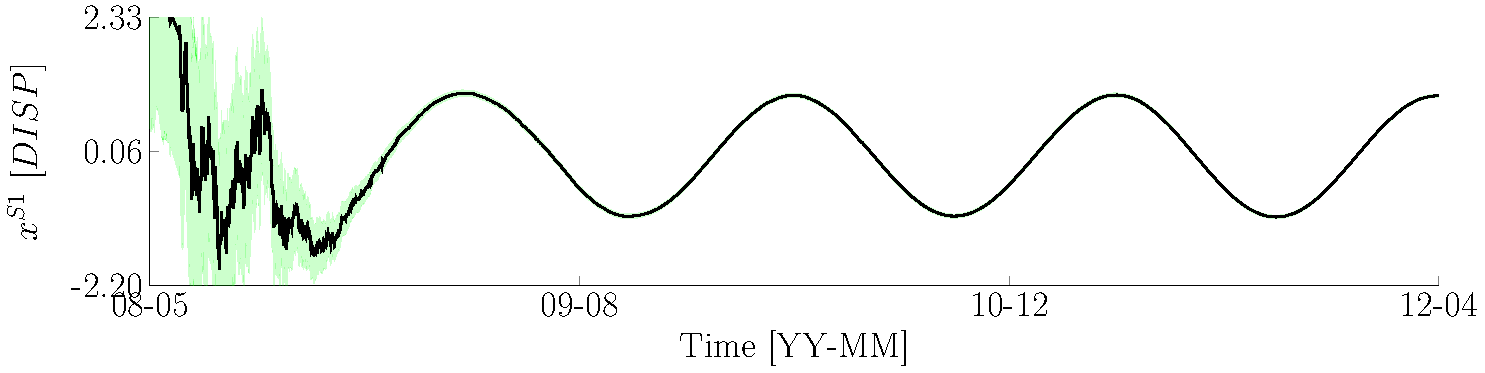
\includegraphics[width=0.9\linewidth]{./docfigs/Example_DISPSIM_ANOMALY/optim_param_default_initialhiddenstate/DISP_S1_4.pdf}
\caption{Estimated displacement yearly periodic component (first hidden state)}
\end{subfigure}
\begin{subfigure}{\linewidth}
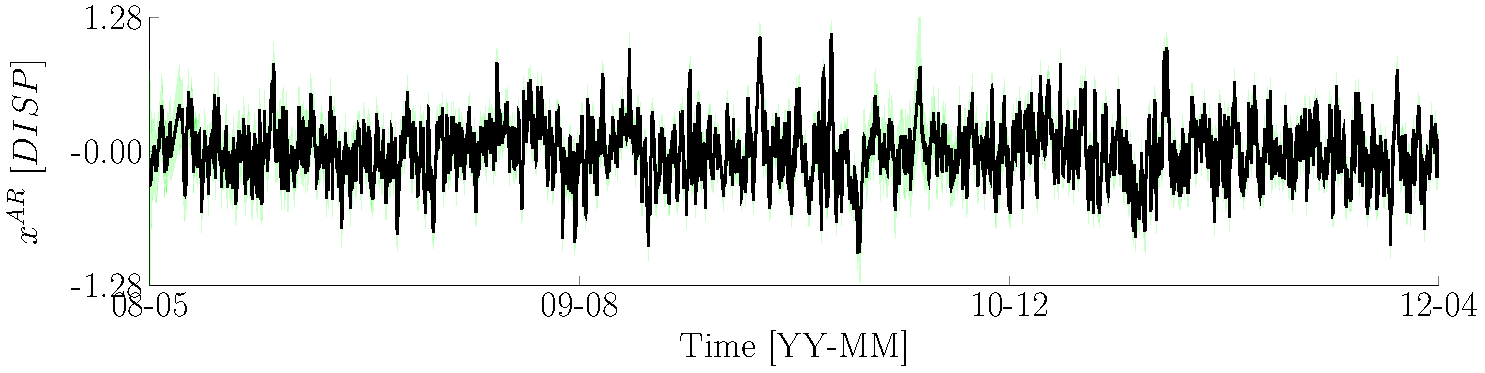
\includegraphics[width=0.9\linewidth]{./docfigs/Example_DISPSIM_ANOMALY/optim_param_default_initialhiddenstate/DISP_AR_6.pdf} 
\caption{Estimated displacement autoregressive component}
\end{subfigure}
\caption{Estimated results using OpenBDLM optimized model parameters and default initial hidden states. The hidden states are estimated from the data presented in Figure~\ref{fig:DataSummaryRaw3}a. The solid line and shaded area represent the mean and standard deviation of the estimated hidden states, respectively.}
\label{fig:DISPSIMANOMALYOptimizedDefaultExample3}
\end{figure*}


\subsection{Step 9: estimate the initial hidden states}


Type \colorbox{light-gray}{\lstinline[basicstyle = \mlttfamily \small, backgroundcolor = \color{light-gray}]!OpenBDLM_main('CFG_Example_DISP_ANOMALY_optim.m');!} in the \MATLAB{} command line.
Then, type  \colorbox{light-gray}{\lstinline[basicstyle = \mlttfamily \small, backgroundcolor = \color{light-gray}]!2!}, to optimize the initial hidden states value.
The optimized initial hidden states mean, covariance  and model probability values for model class 1 are 
\begin{align*}
 \bm \mu^{1,\text{*}}_{0} & = [	-9.43 ,	-0.0109	, -5.03\times 10^{-9}	, 1.08  ,	-0.00634	, -0.548    ]^{\intercal}, \text{and} \\
 \text{diag}(\bm\Sigma^{1,\text{*}}_{0})  & = [	0.139 ,	0.000877,	2.26  	,0.00224	,0.00105,	0.32     ],  \text{and} \\
 \pi_{0}^{1,\text{*}} & = 0.997,
\end{align*}
respectively.
The optimized initial hidden states mean, covariance  and model probability values for model class 2 are 
\begin{align*}
 \bm \mu^{2,\text{*}}_{0} & = [	-9.53 ,	0.102 ,	-0.0599	,  1.08  ,	-0.00636, 	-0.482     ]^{\intercal}, \text{and} \\
 \text{diag}(\bm\Sigma^{2,\text{*}}_{0})  & = [	0.674 	,0.418 ,	0.803 ,	0.00224,	0.00105	, 0.759    ], \text{and} \\
 \pi_{0}^{2,\text{*}} & = 0.00279,
\end{align*}
respectively.
Once it is done, type  \colorbox{light-gray}{\lstinline[basicstyle = \mlttfamily \small, backgroundcolor = \color{light-gray}]!3!}, and then  \colorbox{light-gray}{\lstinline[basicstyle = \mlttfamily \small, backgroundcolor = \color{light-gray}]!1!} to compute the filtered hidden states using the optimized model parameters and optimized initial hidden states.
The value of the log-likelihood is $188$.
The estimated hidden states are presented in Figure~\ref{fig:DISPSIMANOMALYOptimizedOptimizedExample3}.



\begin{figure*}[h!]
\centering
\begin{subfigure}{\linewidth}
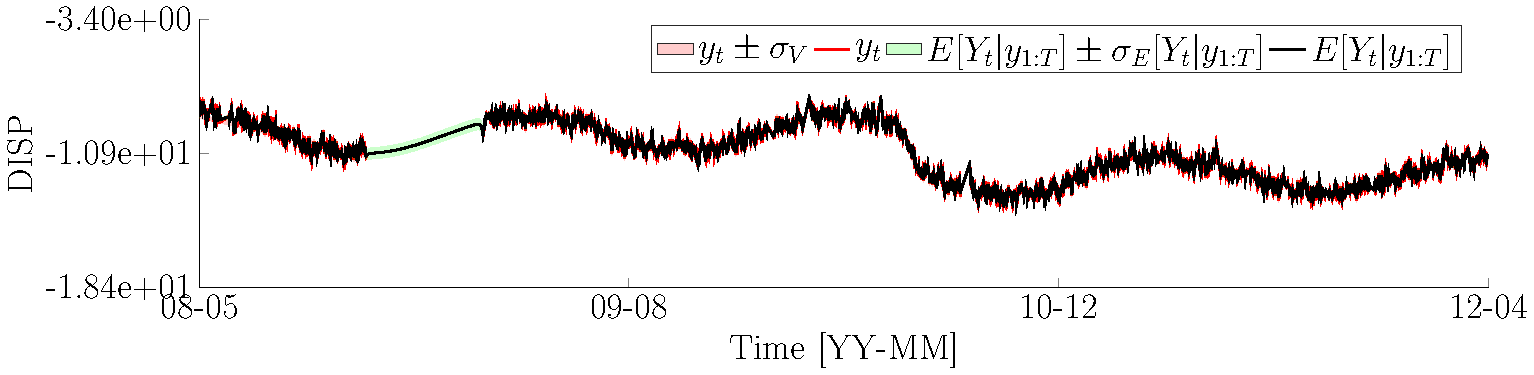
\includegraphics[width=0.9\linewidth]{./docfigs/Example_DISPSIM_ANOMALY/optim_param_optim_initialhiddenstate/DISP_ObservedPredicted.pdf}
\caption{Observed and estimated displacement data}
\end{subfigure}
\begin{subfigure}{\linewidth}
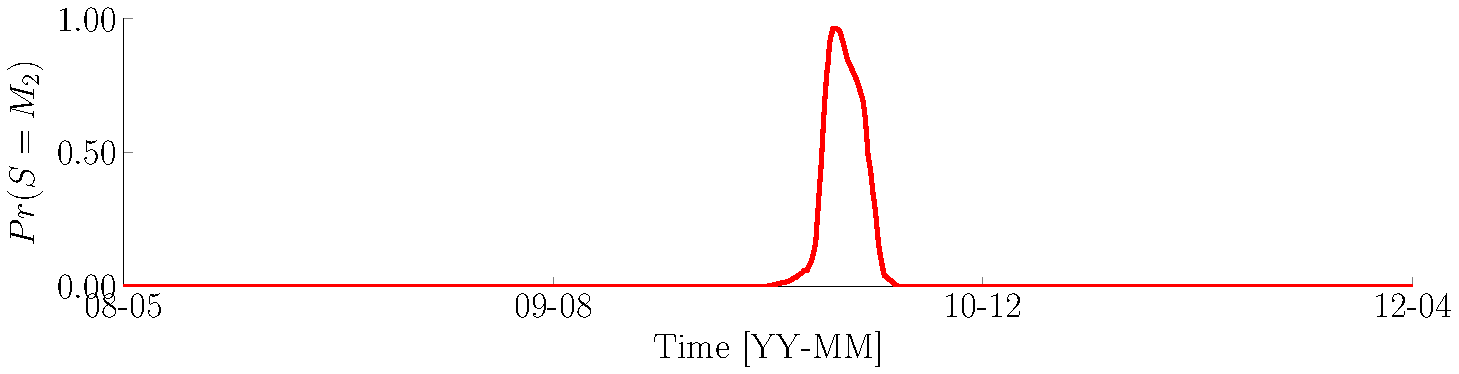
\includegraphics[width=0.9\linewidth]{./docfigs/Example_DISPSIM_ANOMALY/optim_param_optim_initialhiddenstate/ModelProbability.pdf} 
\caption{Estimated probability of anomaly (probability of model class 2)}
\end{subfigure}
\begin{subfigure}{\linewidth}
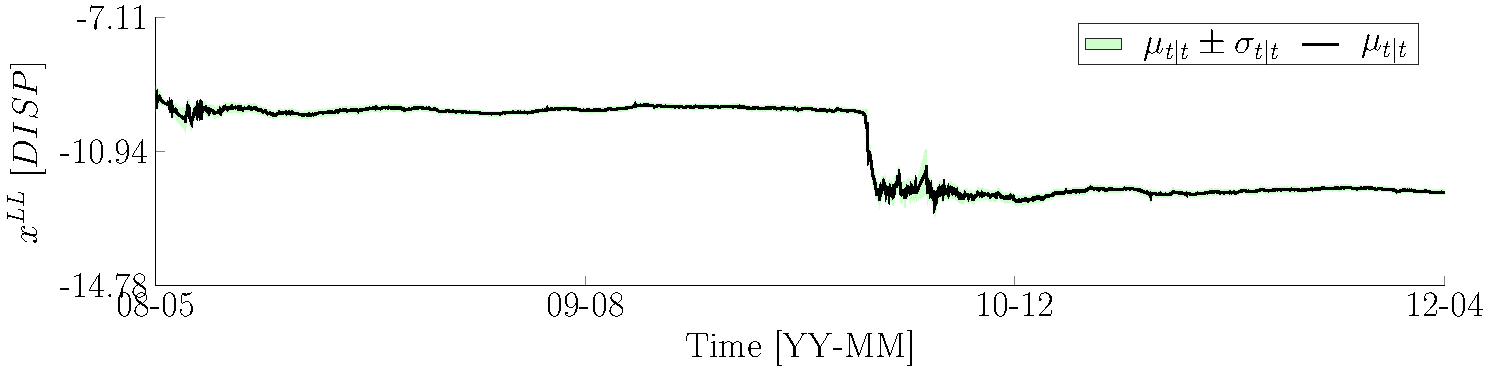
\includegraphics[width=0.9\linewidth]{./docfigs/Example_DISPSIM_ANOMALY/optim_param_optim_initialhiddenstate/DISP_LL_1.pdf} 
\caption{Estimated displacement local level component}
\end{subfigure}
\begin{subfigure}{\linewidth}
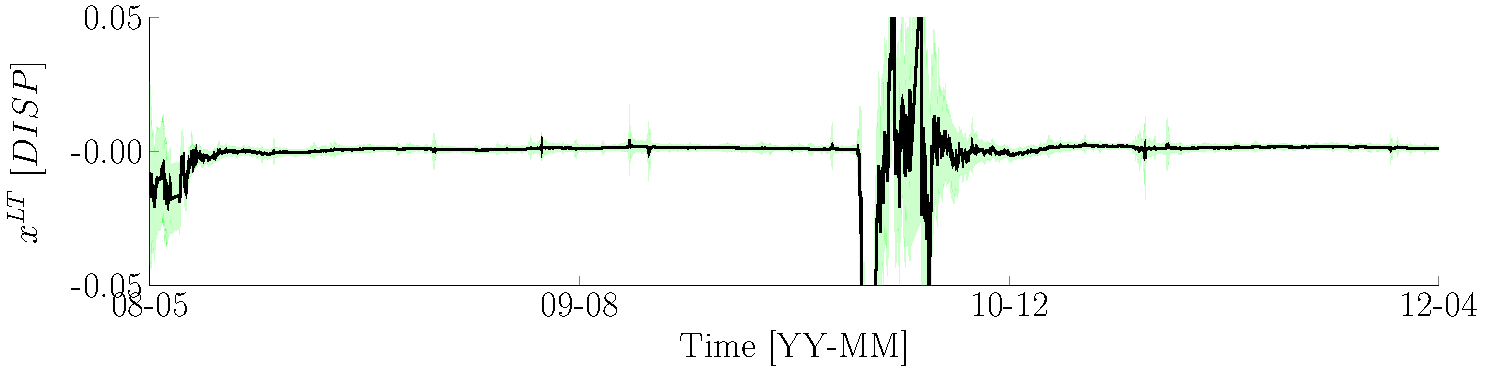
\includegraphics[width=0.9\linewidth]{./docfigs/Example_DISPSIM_ANOMALY/optim_param_optim_initialhiddenstate/DISP_LT_2.pdf}
\caption{Estimated displacement local trend component.}
\end{subfigure}
\begin{subfigure}{\linewidth}
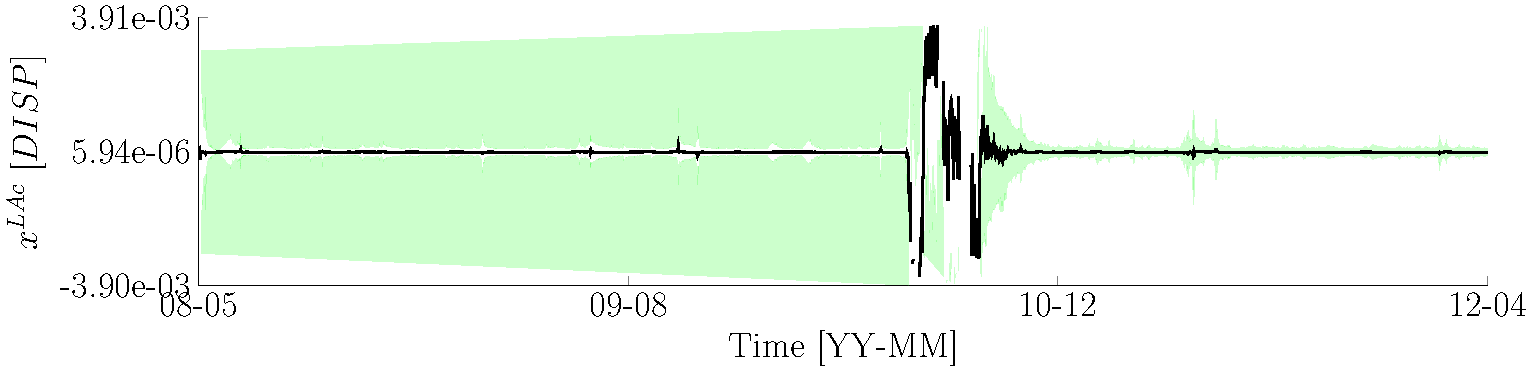
\includegraphics[width=0.9\linewidth]{./docfigs/Example_DISPSIM_ANOMALY/optim_param_optim_initialhiddenstate/DISP_LAc_3.pdf}
\caption{Estimated displacement local acceleration component.}
\end{subfigure}
\end{figure*}
\begin{figure*}[h!]
\ContinuedFloat
\begin{subfigure}{\linewidth}
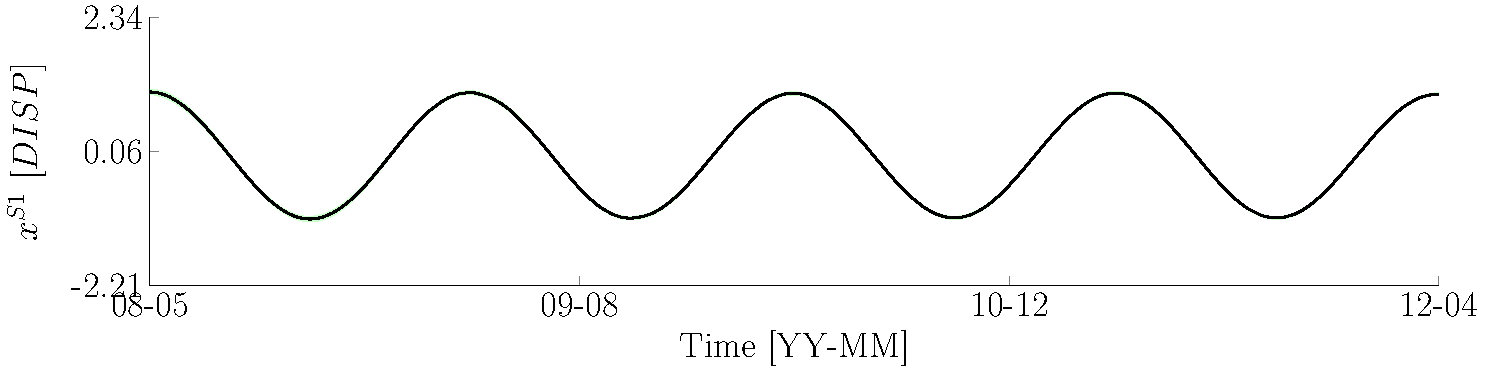
\includegraphics[width=0.9\linewidth]{./docfigs/Example_DISPSIM_ANOMALY/optim_param_optim_initialhiddenstate/DISP_S1_4.pdf}
\caption{Estimated displacement yearly periodic component (first hidden state)}
\end{subfigure}
\begin{subfigure}{\linewidth}
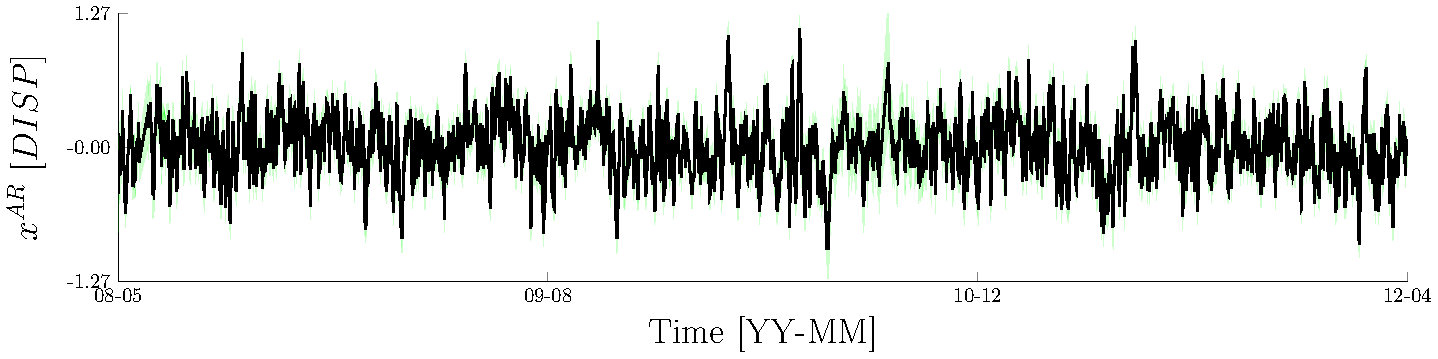
\includegraphics[width=0.9\linewidth]{./docfigs/Example_DISPSIM_ANOMALY/optim_param_optim_initialhiddenstate/DISP_AR_6.pdf} 
\caption{Estimated displacement autoregressive component}
\end{subfigure}
\caption{Estimated results using OpenBDLM optimized model parameters and optimized initial hidden states. The hidden states are estimated from the data presented in Figure~\ref{fig:DataSummaryRaw3}a. The solid line and shaded area represent the mean and standard deviation of the estimated hidden states, respectively.}
\label{fig:DISPSIMANOMALYOptimizedOptimizedExample3}
\end{figure*}
